\section{\acl{LSTM}}
\label{mainsec:lstm}
\textit{Daniel Andrés López, Frank Reichwein}

Eine weitere Art eine Klassifizierung vorzunehmen ist es ein neuronales Netz zu
verwenden. Dieser Ansatz ist durch die Biologie motiviert und lehnt sich an die
Arbeitsweise eines Gehirns an. Im Gehirn sind Neuronen über Synapsen miteinander
verbunden. Nervenbahnen aus dem gesamten Körper erreichen die Neuronen und
stimulieren sie in unterschiedlicher Intensität. Wird dabei ein Schwellwert
überschritten ist dieses Neuron aktiviert und sendet ebenfalls einen Impuls an
die mit ihm über die Synapsen verbundenen Neuronen. Dies geschieht fortlaufend.
Die Synapsen sind jedoch unterschiedlich stark ausgeprägt, um auch eine
unterschiedliche Stimulierungsintensität weiterzugeben. Dies kommt einer
Gewichtung der Neuronen gleich, da die Eingangssignale einen unterschiedlich
starken Einfluss auf das stimulierte Neuron haben. Die Synapsen sind jedoch
nicht fest und von vornherein vorgegeben. Sie werden kontinuierlich auf- und
abgebaut bzw. verändert. Dieser Vorgang wird im Allgemeinen Lernen bezeichnet.
Die erlebten Erfahrungen werden in dem Netz von Neuronen und Synapsen
verarbeitet und dadurch gespeichert. Erreichen das Gehirn nun neue
Sinneseindrücke werden die Neuronen erneut stimuliert und je nach Ergebnis
werden bestimmte Erinnerungen, Gefühle, Aktionen oder anderes erlebt und 
ausgeführt. Jedoch sind sie nicht direkt an ein bestimmtes Ereignis geknüpft,
sondern wurden durch verschiedene Erfahrungen verallgemeinert, um so
verschiedenen Situationen gut verarbeiten zu können.
 
\paragraph{Modelle von Neuronen und Synapsen}
Im Bereich des maschinellen Lernen wird versucht die Funktionsweise eines
Gehirns bzw. Netzes aus Neuronen und Synapsen nachzubilden. Dies wird durch
vereinfachte Modelle von Neuronen und Synapsen erreicht. Ein einfaches Modell
wird hier als Grundlage verwendet. Es ist das Modell von McCulloch und Pitts von
1943 (vgl. \cite{Mcc43}) und modelliert ein Neuron mit $n$-vielen Eingabewerten
($x_1,\ldots,x_n$) und einem Ausgabewert $y$. Die Eingabewerte entsprechen der
Aktivierung eines Vorgängerneurons und der Ausgabewert der Aktivierung des
betrachteten Neurons.
\begin{figure}[htbp]
    \centering
   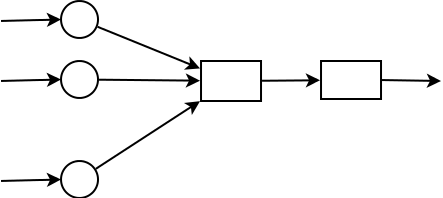
\includegraphics[width=0.9\columnwidth]{lstm/neuron}
\caption{Modell eines McCulloch and Pitt Neurons}
\label{fig:neuron}
\end{figure}  
Die \autoref{fig:neuron} zeigt den Aufbau eines solchen Neurons. Die Eingaben
werden dabei zuerst im \textit{Addierer} summiert, eine Schwellwertfunktion (bzw.
allgemeiner eine Aktivierungsfunktion) bestimmt dann mit der Summe den
Ausgabewert (die Aktivierung) des Neurons. Des Weiteren werden auch die Synapsen
nachgebildet in dem jeder Eingabewert bei der Summierung individuell mit $w_i$
gewichtet wird. Die Gewichte entsprechen den unterschiedlich stark ausgeprägten
Synapsen.
Das klassische Modell erlaubt nur binäre Ein- und Ausgaben, dies kann jedoch auf
reelle Zahlen erweitert werden, um unterschiedlich starke Stimulierungen bzw.
auch negative Werte (Hemmungen) zuzulassen.

\paragraph{Neuronale Netzwerke}
Einzelne Neuronen können allerdings kein Gehirn nachbilden. Aus diesem Grund ist
die Kombination mehrerer Neuronen zu einem neuronalen Netz nötig. Im einfachsten
Fall entsteht dabei ein \textit{Perzeptron} (vgl.
\cite{rosenblatt58a,1165576}). Es werden $n$-viele Neuronen verwendet. Alle
Eingaben werden von allen Neuronen verarbeitet und jedes Neuron hat eine eigene
Aktivierung. Die Gewichte (Synapsen) sind individuell für jedes Neuron. Die
Ausgaben ergeben den Ausgabevektor $\bf{y}$ des Netzwerkes. Um komplexere
Sachverhalte darstellen zu können, ist es nötig Neuronen in Abhängigkeit
voneinander zu betrachten. Dies wird in \acp{MLP} vorgenommen \cite{1165576}.
Mehrere Perzeptrons werden hintereinandergeschaltet, sodass die Ausgabe des
einen Perzeptrons (ein Layer) die Eingabe des nächsten Perzeptrons ist (vgl.
\autoref{fig:mlp}).
\begin{figure}[htbp]
    \centering
   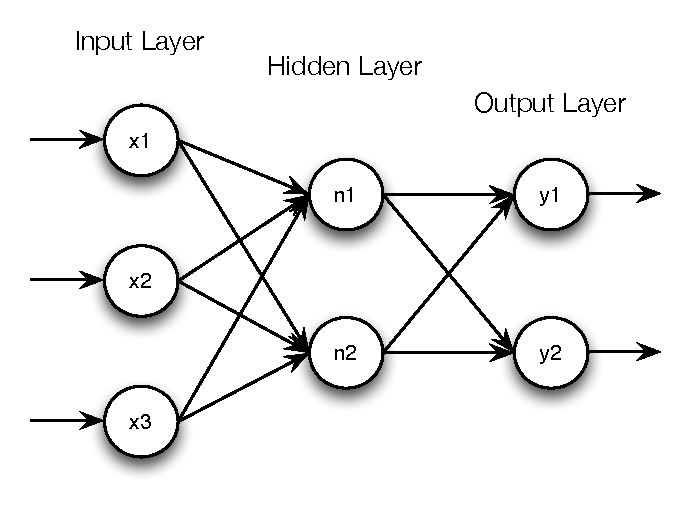
\includegraphics[height=50mm]{lstm/mlp}
\caption{MLP-Netz}
\label{fig:mlp}
\end{figure}
Lediglich die Ausgabe des letzten Perzeptrons ist die Ausgabe des Netzwerks.
Ein Netzwerk kann als gerichteter Graph dargestellt werden. Die Richtung
entspricht dem Datenfluss. Perzeptrons und \acp{MLP} sind azyklische Graphen,
d.h. die Verbindungen von Neuronen gehen nur in Vorwärtsrichtung und bilden
somit keinen Kreis. Daher werden diese Netzwerke \textit{Feedforward}-Netzwerke
genannt. Um besser die Funktionsweise von Gehirnen nachzubilden ist es notwendig
auch Verbindungen von Neuronen auf sich selbst zuzulassen. Somit entsteht ein
zyklischer Graph und das Netzwerk wird zu einem Rekurrenten Neuronalen Netz
(\acsu{RNN}). \cite{RainerSchmoll2006}

Im Rahmen dieses Kapitels wird erläutert, wie \acsp{LSTM}, eine spezielle Form
von \acp{RNN}, zur Klassifikation von Gesten des schallbasierten Dopplereffekts
genutzt werden können. Dazu wird zuerst darauf eingegangen wie ein \ac{LSTM} im
Allgemeinen funktioniert und wie ein solches Netzwerk trainiert werden kann.
Darauf aufbauend wird das Verfahren auf das Projekt angepasst. Es werden die
Datenaufbereitung, die Anpassung des Klassifikators, die Implementierung in
Python, das Training und eine Evaluierung besprochen.


\subsection{Funktionsweise des Klassifikators (Allgemein)}
\label{sec:lstm_allg}
Ein \acl{LSTM} ist ein spezielles \ac{RNN}. Es wurde 1997
vorgestellt\cite{Hochreiter:1997}. Wie allgemein Neuronale Netze und
insbesondere \ac{RNN} können auch \ac{LSTM}-Netze biologisch motiviert werden.
Neuronen im Gehirn verhalten sich nicht mit der gleichen Eingabe gleich.
Vielmehr reagieren sie abhängig von verschiedenen Situationen anders. Beeinflusst
wird dies durch vorangegangene Ereignisse. Eindrücke (Eingaben) werden so in
einen zeitlichen Bezug gestellt und dadurch entsteht eine zusammenhängende
Erinnerung. Diese wird wie eine einzelne Eingabe ebenfalls generalisiert in den
Synapsen und Neuronen gespeichert. Mit Hilfe der \ac{LSTM} Architektur wird
versucht dieses Verhalten nachzuahmen.

In einem Netz mit \ac{LSTM}-Einheiten sind diese keine einzelnen Neuronen
sondern Blöcke aus mehreren Neuronen und Toren (ein Tor bzw. engl.
Gate bestimmt ob ein anliegender Wert weitergegeben wird oder nicht).
Die Blöcke werden im Netz wie ein Neuron behandelt. Sie erhalten alle Eingaben
und geben einen Wert aus. \ac{LSTM}-Layer werden in der Regel als Hidden-Layer
in einer \ac{MLP}-Architektur eingesetzt, jedoch ist kein weiteres Hidden-Layer
nötig. Für das Ausgabe-Layer werden je nach Problemstellung unterschiedliche
Arten verwendet, z.B. lineare, sigmoidale oder Softmax-Layer.

\paragraph{\ac{LSTM}-Block}

\begin{figure*}[htfp]
	\begin{center}
	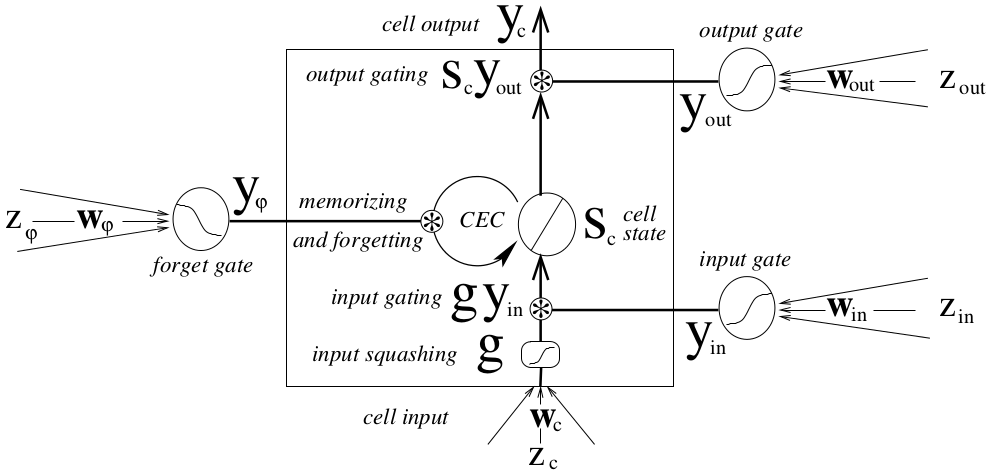
\includegraphics[width=0.8\textwidth]{lstm/lstm_block_formulas}
	\caption[\acs{LSTM} Block]{\acs{LSTM} Block mit einer Memoryzelle ohne
	Peepholes} \tiny Quelle: \cite{Gers2002b}
	\label{fig:lstm_block}
	\end{center}
\end{figure*}  

\autoref{fig:lstm_block} zeigt den schematischen Aufbau eines \ac{LSTM}-Blocks
nach \cite{Gers2002b}. Der Block besteht dabei aus mehreren Komponenten. Diese
werden anhand ihrer Berechnung bei einem \textit{vorwärts} Durchlauf der Daten
erläutert.
\begin{itemize}
	\item Eingabewerte $y_m(t-1)$
	\item Zelleingang $z_c$ berechnet durch \autoref{eq_lstm_in}
	\item Inputgate $z_{in}$ berechnet nach \autoref{eq_lstm_gate}
	\item Forgetgate $z_\varphi$ berechnet durch \autoref{eq_lstm_gate}
	\item Memoryzelle mit dem aktuellen Wert $s_c$ berechnet durch
	\autoref{eq_lstm_cs}
	\item Outputgate $z_{out}$ berechnet nach \autoref{eq_lstm_gate}
	\item Ausgabewert $y_m(t)$ berechnet durch \autoref{eq_lstm_out}
\end{itemize}

% Inputs
\begin{equation}
\label{eq_lstm_in}
z_{c}(t) = \sum \limits_{m} w_{c,m}y_m(t-1)
\end{equation}

% Gate Allgemein
\begin{equation}
\label{eq_lstm_gate}
\begin{split}
y_{gate}(t) &= f_{gate}(z_{gate}(t))\\
z_{gate}(t) &= \sum \limits_{m} w_{gate,m}y_m(t-1)\\
gate &\in \{in,\varphi,out\}
\end{split}
\end{equation}

% Cell State
\begin{equation}
\label{eq_lstm_cs}
\begin{split}
s_{c}(0) &= 0\\
s_{c}(t) &= y_{\varphi}(t)s_{c}(t-1) +
y_{in}(t)g(z_{c}(t))
\end{split}
\end{equation}

% Output
\begin{equation}
\label{eq_lstm_out}
\begin{split}
y_{c}(t) &= y_{out}(t)s_{c}(t)\\
\end{split}
\end{equation}

Die Funktionen $f_{in}$, $f_{\varphi}$ und $f_{out}$ sind sigmoidale Squashing
Funktionen, die Eingabewerte an den Gates auf $y\approx1$ oder $y\approx0$
zusammenfassen. Dies hat zur Folge, dass an den \textit{gating} Stellen Werte
gelöscht (bei $y\approx0$) oder unverändert durchgelassen werden (bei
$y\approx1$). Somit kontrolliert das Inputgate (\autoref{eq_lstm_cs} zweiter
Teil, zweiter Summand), ob neue Werte die Memoryzelle erreichen, das Forgetgate
(\autoref{eq_lstm_cs} zweiter Teil vorne), ob der vorherige Zustand erhalten
bleibt oder nicht berücksichtigt wird und das Outputgate (\autoref{eq_lstm_out})
wann ein Zustand der Memoryzelle ausgegeben wird. Grundsätzlich hat jeder
Eingang in den \ac{LSTM}-Block inklusive der Eingänge der Gates ein eigenes
Gewicht. Diese sind mit $w_{i,m}$ benannt, wobei $i$ der Eingang oder das Gate
repräsentiert und $m$ der Index über die Eingabedimension ist. Daher hat ein
\ac{LSTM}-Block $4\cdot Eingabedimension$ viele Gewichte. 

\acp{LSTM} werden durch ihre autorekurrente Verbindung der Memoryzelle zu
\acp{RNN}. Diese rekurrente Verbindung ist besonders, da sie beim Training
Fehler nicht vor in die komplette Vergangenheit zurück propagiert. Erreicht wird
das durch ein Gewicht der Verbindung von $1.0$ (\autoref{eq_lstm_cs}). Das zuvor
beschriebene Forgetgate nimmt Einfluss auf dieses Gewicht. Soll der Wert
$s_c(t-1)$ in der Berechnung nicht berücksichtigt werden, setzt das Gate das
Gewicht auf $\approx0$ andernfalls behält es den aktuellen Wert des Gewichts mit
$\approx1$ bei. 

Eine Erweiterung zu dem vorgestellten \ac{LSTM}-Block sind zusätzlich weitere
rekurrente Verbindungen (vgl. \cite{Gers2002b}). Diese weiteren rekurrenten
Verbindungen werden \textit{Peepholes} genannt und verbinden die die Memoryzelle
zusätzlich zu den Gates, sodass sich die \autoref{eq_lstm_gate} für die Gateaktivierung
wie folgt ändert:
% Gate Allgemein
\begin{equation}
\label{eq_lstm_gate_peephole}
\begin{split}
z_{gate}(t) &= \sum \limits_{m} w_{gate,m}y_m(t-1) \\
			&+ w_{gate,c} s_c(t-1)
\end{split}
\end{equation}

$w_{gate,c}$ ist dabei das Gewicht der rekurrenten Verbindung von der
Memoryzelle zum Gate. Peepholeverbindungen machen auf diese Art die Information
der Memoryzelle den Gates verfügbar und können so das Netzwerk verbessern
\cite{Gers2002b}. 

Der beschriebene \ac{LSTM}-Block enthält eine einzelne Memoryzelle. Denkbar sind
jedoch Blöcke mit mehreren Memoryzellen, die sich dann die die drei Gates
teilen. Auch sind hier Peepholeverbindungen möglich, die Gates berücksichtigen
dann alle Werte der Memoryzellen. Dieser Ansatz wird in der Ausarbeitung nicht
weiter betrachtet. Weitere Informationen sind unter anderem in \cite{GERS2001}
zu finden.

\paragraph{Training eines \ac{LSTM} Netzes}
Damit neuronale Netze (damit auch \ac{LSTM}-Netze) ein gutes Ergebnis liefern
müssen ihre Gewichte auf das Problem angepasst sein. Es ist jedoch nicht einfach
berechenbar wie die korrekten problembezogenen Gewichte sind. Daher müssen sie
iterativ verbessert werden. Dieser Vorgang wird Training genannt. Dabei werden
einem zufällig initialisierten Netzwerk Datensätze zum Klassifizieren gezeigt.
Das Netzwerk liefert daraufhin ein Ergebnis. Das gewonnene Ergebnis wird mit dem
Zielergebnis verglichen. So lässt sich eine Fehlerquote berechnen. Es gibt
verschiedene Verfahren wie die Fehlerquote die Gewichte bzw. das Netz
beeinflusst, um in der nächsten Iteration eine geringere Fehlerquote zu
erhalten. Nachfolgend werden die Grundideen von zwei verschiedenen
Trainingsansätzen erläutert:
\begin{itemize}
	\item Fehlerrückführung (engl. Backpropagation)
	\item Evolutionsbasiertes Training
\end{itemize}

\subparagraph{Backpropagation}
Das Verfahren \textit{Fehlerrückführung} ist ein Gradientenabstiegsverfahren.
Das bedeutet, es versucht die Fehlerquote als Ergebnis einer Funktion des Netzes
aufzufassen und diesen Wert daran zu minimieren. Dabei werden in Richtung des
Gradienten der Funktion die Gewichte in kleinen Schritten angepasst. Die
Anpassung der Gewichte erfolgt im sog.
\textit{Backward-Pass} des Netzes. Der Fehler wird durch das Netz rückwärts
gereicht und dabei sukzessive die Gewichte angepasst. Das Problem, das jedoch
auftritt, ist, dass dieses Verfahren nicht gegen 0 konvergieren muss, denn es
wird entlang eines Gradienten optimiert, der auch zu einem lokalen Minima führen
kann. Außerdem ist es möglich über Minima hin wegzuoptimieren und das Ergebnis
so wieder zu verschlechtern. Um dies zu verhindern gibt es verschiedene
Methoden, welche hier nicht weiter erläutert werden. Für \ac{LSTM}-Netze ist
eine Erweiterung des Backpropagation Algorithmus sinnvoll:
\acl{RProp} (elastische Fortpflanzung, \acsu{RProp}). Für die erweiterte Form
kann sogar eine globale Konvergenz bewiesen werden. Des Weiteren liefert er im
Allgemeinen Konvergenz schneller als Backpropagation. Jedoch besteht auch hier
die Gefahr, dass ein lokales Minima übersprungen wird. Dies ist von Bedeutung,
da ein globales Minima evtl. eine zu hohe Trainingszeit erfordert und deshalb
lokale Minima gesucht werden. Der wesentliche Unterschied von \ac{RProp} zu
Backpropagation besteht darin, dass \ac{RProp} die vorherige Gewichtsänderung
mit in die aktuelle Änderung mit einfließen lässt. Bei Backpropagation ist dies
nicht der Fall. Weitere Informationen zu diesen Verfahren und deren konkreten
Umsetzungen durch \textit{Backprogation through time (BPTT)} und \textit{Real
Time Recurrent Learning (RTRL)} sind in
\cite{RainerSchmoll2006,Gers2002b,GERS2001} zu finden.

\subparagraph{Evolutionsbasiertes Training}
Die Idee des evolutionären Trainings ist wie neuronale Netze biologisch
motiviert. Eine Population mutiert bzw. pflanzt sich fort (Kombination von
spezifischen Eigenschaften, Genom). Dabei wird jedoch eine \textit{Fitness}
Funktion angewendet, sodass die Fitness des Genoms mit jeder Generationsstufe
(Veränderungsschritt) ein besseres Ergebnis liefert. \cite{Marsland} Dieser
Mechanismus der Evolution eines Genoms wird mit Hilfe verschiedener Algorithmen
wie dem \textit{Genetischen Algorithmus} versucht nachzuahmen. Wichtig ist
dabei, dass eine geeignete Repräsentation des Netzwerkes durch ein Genom
gefunden, eine problemspezifische Fitness Funktion genutzt und die Population
sich in einer sinnvollen Art und Weise verändert. Dieser Ansatz wird in
\cite{Schmidhuber05evolino:hybrid} mit dem \textit{Evolino} Algorithmus
(Evolution of recurrent systems with Linear outputs) umgesetzt. Evolutionäres
Lernen wird hier nicht weiter betrachtet, da es nicht genutzt werden kann (vgl.
\autoref{sec:lstm_training}).


\subsection{Anwendung auf Projekt}
Für das Projekt wird ein LSTM-Netz erstellt welches aus folgenden Schichten besteht:

\begin{itemize}
\item \textbf{Input Layer} Für die Annahme der Daten.
\item \textbf{Hidden-Layer} Besteht aus LSTM-Blöcken.
\item \textbf{Output Layer} Das Output Layer besteht aus Neuronen, die die 
Softmax Funktion als Aktivierungsfunktion verwenden.
\end{itemize}

\begin{figure}[htbp]
    \centering
   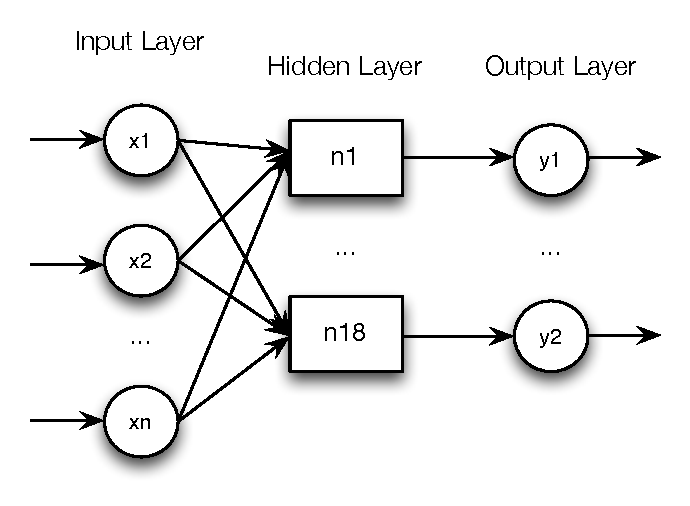
\includegraphics[height=50mm]{lstm/lstm_netz}
\caption{LSTM-Netz}
\label{fig:lstm_netz}
\end{figure}
Die genaue Anzahl der Neuronen für das Input- und Hidden-Layer stand zu Beginn
des Projektes nicht fest. Sie wurde durch Tests, die in \autoref{sec:lstm_data}
beschrieben sind, ermittelt. Die Anzahl der Neuronen in dem Output-Layer ergab
sich aus der Anzahl der Gesten. Es ist üblich für jedes Ergebnis ein eigenes
Output-Neuron zu erstellen.

\subsubsection{Datenaufbereitung}
\label{sec:lstm_data} 

In \autoref{sec:intro} wird beschrieben wie die Daten aufgenommen und im
Allgemeinen verarbeitet werden, bevor sie den Klassifikatoren zur Verfügung
gestellt werden. Diese erhalten jeweils einzelne Frames mit je 64 Daten. Die
Daten entsprechen dem Frequenzspektrum im Umfeld der Referenzfrequenz von
$18500\text{kHz}$. Eine Geste wurde mit 32 Frames aufgenommen. Für
\ac{LSTM}-Netzwerke sind diese rohen Daten eher ungeeignet. Die Netzwerke können
zwar im Allgemeinen mit unverarbeiteten Daten umgehen, trotzdem ist ein
Vorverarbeitung sinnvoll, da sich dadurch die Verallgemeinerung des Problems
verbessert, die Trainingszeit verkürzt und die benötigten Beispiele verringern
\cite{RainerSchmoll2006}. Aus diesen Gründen wird eine Vorverarbeitung der Daten
vorgenommen.

Die Beispieldaten sind auf verschiedenen Hardwareplattformen mit
unterschiedlichen Lautstärke und Aufnahmelautstärke Konfigurationen erzeugt
worden. Der Wertebereich dieser Daten ist somit groß und unterschiedlich bei
gleichen Gesten. Das Problem dass durch diese Varianz der Wertemenge entsteht
ist, dass \acp{LSTM} Netze (bzw. jede Form von neuronalen Netzen) die Gewichte
entsprechend groß kalibrieren muss, um Unterschiede ausgleichen zu können und
eine verallgemeinertes Ergebnis zu liefern. Da jedoch das (später beschriebene)
Trainingsverfahren iterativ die Gewichte in kleinen Schritten anpasst, führen
große Gewichte zu einem hohen Trainingsaufwand. Um dies zu vermeiden werden die
Daten normalisiert. Konkret wird dabei der Maximalwert eines Frames als
Normierungsfaktor gewählt. Dadurch liegen alle Werte im Intervall $[0,1]$.
Eine Transformation des Spektrums wird druch die Differenz zum Ruhespektrum
vorgenommen. Dazu wird der allgemeine Ruhezustand aus den Beispielen (Geste 6
und 7) durch das normalisierte Mittel gewonnen und dann von jedem Beispiel
abgezogen. Es werden hierbei lediglich die Beispiele verwendet, denkbar ist
jedoch auch die Aufnahme des Ruhezustands auf dem Zielgerät, um spezifischere
Daten zu erhalten.

Bei der Betrachtung der Daten fällt auf, dass der Doppler-Effekt in einem
kleinen Intervall um die Referenzfrequenz auftritt und die Daten außerhalb
dieses Intervalls keine große Bedeutung spielen. Aus diesem Grund ist eine
Verkleinerung der Frame Größe in Betracht zu ziehen. Da jedoch eine manuelle
Betrachtung aller Daten nicht möglich ist, lässt sich diese Beobachtung nicht
manuell verifizieren. Daher werden mehrere \ac{LSTM}-Netze mit unterschiedlichen
Inputdimensionen trainiert und die Ergebnisse verglichen (vgl. Anhang
\autoref{tab:inputtests}). Erstaunlicherweise ist die aufgestellte Vermutung falsch
und die Netzwerke ohne zugeschnittenen Trainingsdaten klassifizieren besser.

Eine weitere Beobachtung die gemacht werden kann ist, dass benachbarte
Datenpunkte sich nicht wesentlich unterscheiden. Dies kann genutzt werden um die
Eingabedimension zu verringern, indem z.B. jeweils zwei benachbarte Datenpunkte
miteinander addiert werden. Dies kann auch mit dem verkleinern der Frames
kombiniert werden. Um den Einfluss auf das Klassifizierungsverhalten von
\ac{LSTM}-Netzen zu zeigen sind auch hier Tests durchgeführt worden (vgl. Anhang
\autoref{tab:inputtests}). Das Ergebnis zeigt, dass die Netze ohne
die Summe benachbarter Werte besser klassifizieren als mit der Summe. 

Weitere Methoden der Datenvorverarbeitung wurden ebenfalls untersucht, jedoch
hat dies die Ergebnisse ebenfalls negativ beeinflusst, weshalb sie nicht näher
betrachtet wurden. Darunter fällt u.a. die statische Eliminierung von Rauschen.
Diese Methode setzt jeden Wert der unter einem bestimmten Schwellwert ist zu 0,
da dies kein signifikanter Beitrag zur Geste ist sondern ein Rauschen. Das
Ergebnis dieser Untersuchung zeigt jedoch keinen positiven Effekt auf die Fehlererkennungsrate, sodass die Idee nicht
genutzt wird (vgl. \autoref{tab:noiseremovingtests}).
 
\begin{table}[h]
\centering
\begin{tabular}{|c|c|c|c|}
\hline
\textbf{Rausch-} & keine & \textless 0,0125 & \textless 0,025\\
\textbf{entfernung}&&&\\
 \hline
\textbf{Fehlerrate}&31,83\%&47,87\%&57,59\%\\\hline
\end{tabular} 
\caption[Tests für Rauschentfernung]{Tests um den Einfluss von Rauschentfernung zu untersuchen. Das Trainingsverfahren ist \texttt{RProp}. Die Anzahl der LSTM-Blöcke ist 16. Iterationen 100.}
\label{tab:noiseremovingtests}
\end{table}
 
\subsubsection{Anpassung des Klassifikators}
Das \ac{LSTM}-Netz wird mit Hilfe der Python Bibliothek \texttt{PyBrain}
\cite{schaul2010} erstellt. Diese Bibliothek stellt verschiedene Machine
Learning Algorithmen bereit, unter anderem Neuronale Netzwerke mit
\ac{LSTM}-Neuronen. Des Weiteren sind verschiedene Algorithmen zum Training und
Module zur Nutzung der Netzwerke bereitgestellt. Aufgrund der Beschränkungen der
Bibliothek werden nur \ac{LSTM}-Blöcke mit einer einzelnen Memoryzelle
verwendet. Die verschiedenen Parameter zur Erstellung (Anzahl der
\ac{LSTM}-Blöcke, Anzahl der Ausgabeneuronen, Nutzung von Peepholes, etc.) sowie
die Parameter zur Vorverarbeitung (vgl. \autoref{sec:lstm_data}) werden anhand
von Tests ermittelt, denn eine Berechnung der optimalen Parameter ist nicht
möglich. In den weiteren Kapiteln wird auf die unterschiedlichen Parameter noch
einmal im Detail eingegangen. 


\subsubsection{Implementierung}
Da es zum Ende des Projektes ein Programm geben soll, indem alle Klassifikatoren
eingebunden sind, haben sich alle Teilnehmer auf ein Interface geeinigt, was
jeder Klassifikator implementieren muss. Dies ist die abstrakte Klasse
\texttt{IClassifier}. Die Implementierung des \ac{LSTM}-Klassifikators ist in
der Klasse LSTM zu finden, diese dient als Wrapper-Klasse. Ein Klassendiagramm
ist in \autoref{fig:lstm_class} dargestellt. Die \textit{LSTM}-Klasse enthält je eine Instanz von: 
\begin{itemize}
\item \textit{LSTMClassify}: Enthält die verschiedenen Methode für die Live-Klassifizierung.
\item \textit{LSTMData}: Ist für das speichern und laden der Datensets zuständig.
\item \textit{LSTMNet}: Erstellt, lädt, aktiviert oder speichert ein LSTM-Netz.
\item \textit{LSTMTrain}: Trainiert ein mit verschiedenen Algorithmen das LSTM-Netz.
\end{itemize}
Außerdem wurden in der Datei \texttt{util.py} verschiedene Hilfsfunktionen
erstellt.
Des weiteren werden Konfigurationseinstellungen in einer Datei gespeichert und
zur Initialisierung der geladen.
Da beabsichtigt ist mit dem Programm den PC zu steuern, wurde die Python
Bibliothek \textit{Python-uinput} eingebunden. Mit dieser können
Keycodes an den Kernel geschickt werden.
Die Bibliothek funktioniert nur unter Linux und erfordert Root-Rechte.
Im folgenden wird auf die Implementation der einzelnen Methoden der
\textit{LSTM}-Klasse eingegangen.

\subsubsection*{Live Klassifikation}
Für die Live Klassifikation wurde verschiedene Ideen implementiert. 
Bei allen wird zuerst die \textit{classify} Methode der LSTM-Klasse 
aufgerufen. Diese bekommt den Datensatz der aktuellen Aufnahme übergeben. 
Der Datensatz enthält ein Array mit 64-Datenpunkten. Die übergebenen Daten werden 
Normalisiert und anschließend wird der Durchschnitt abgezogen, wie in Kapitel 
\autoref{sec:lstm_data} beschrieben. Nachdem die Daten vorverarbeitet wurden, 
werden diese einer der verschiedenen\textit{classify}-Methoden übergeben. 

Die Methode \textit{classify1} speichert so lange die übergebenen Datenwerte, 
bis 32-Werte aufgenommen wurden. Diese 32-Werten werden dem \ac{LSTM}-Netz 
übergeben und eine Klassifikation gestartet. Da es bei diesem Ansatz passieren kann, 
dass eine Geste nicht komplett in diesen 32-Werte enthalten ist, wurde ein zweite 
Idee umgesetzt, welche in der Methode \textit{classify2} umgesetzt ist.

Die Methode \textit{classify2} speichert so lange die übergebenen Datenwerte, 
bis 32-Werte aufgenommen wurden. Diese 32-Werten werden dem \ac{LSTM}-Netz 
übergeben und eine Klassifikation gestartet. Die erkannte Geste wird in einer 
Liste gespeichert. Von dieser Liste wird, mittels der Python-Funktion \texttt{mode}, 
der Wert ermittelt der am häufigsten vorkommt. Ist dieser Wert größer als eine 
definierte Schranke wird er in \textit{previouspredict} gespeichert. Wenn vier 
mal hinter einander die gleiche Geste erkannt wurde, wird diese ausgegeben.

Eine weitere Idee besteht darin, die Geste zwischen zwei mal der Geste 6 zu 
suchen. Dies wird in \textit{classify3} versucht.

Da von jedem Datensatz der Durchschnitt abgezogen wird, erscheint sobald eine 
Bewegung statt findet, ein Ausschlag. Diesen zu erkennen wird in \textit{classify4} 
versucht. Bei dieser Implementierung muss der Ausschlag einen bestimmten Schwellwert 
überschreiten und wird anschließend dem LSTM-Netz übergeben.

Bei der Methode \textit{classify5} wird genau so vorgegangen wie bei der vierten 
Idee, es werden aber nicht ab dem Beginn des Ausschlags die Daten an das 
Netz übergeben, sondern mit einem Puffer gearbeitet und wenn eine Ausschlag erkannt 
werden die nächsten 22-Datensätze und 10-Datensätze aus dem Puffer übergeben.

\subsubsection{Training}
\label{sec:lstm_training}
Das Training des \ac{RNN} mit \ac{LSTM}-Blöcken erfolgt mit den in
\autoref{sec:lstm_allg} erläuterten Verfahren in optimierten Version.
\texttt{PyBrain} bietet dazu die Gradientenabstiegsverfahren
\textit{Backpropagation} und \textit{\ac{RProp}}, diverse evolutionsbasierende
Optimierungsverfahren wie \textit{Genetische Algorithmen} oder
\textit{HillClimber} Verfahren und ein Modul zum gradientenbasierenden
\textit{Cross-Validierungsverfahren} an. Mit Hilfe dieser Verfahren kann das
Netzwerk iterativ trainiert werden. Aufgrund von Inkompatibilitäten mit
\ac{LSTM}-Netzwerken sind evolutionsbasierende und crossvalidierende Verfahren
nicht geeignet. Der Fokus des Trainings liegt deshalb auf den
Gradientenabstiegsverfahren. Wie oben beschrieben ist \ac{RProp} eine
Weiterentwicklung von Backpropagation, welche im Gegensatz zur Fehlerrückführung
stabiles Konvergenzverhalten zeigt. Dies wurde mit einer kleinen Testreihe
bestätigt, welche zeigt, dass Backpropagation schwankende Ergebnisse liefert
(vgl. \autoref{tab:backproptests}). Aus diesem Grund wird das Training nur mit
\ac{RProp} durchgeführt.
 
Das Training eines \ac{LSTM}-Netzes ist in der Regel \texttt{supervised}.
PyBrain bietet daher die Möglichkeit Datasets für die Klassifikation von
Sequenzen an. Dieses wird mit den Daten und den zugehörigen Klassen erstellt.
Die werden zuvor noch wie in \autoref{sec:lstm_data} beschrieben vorverarbeitet.
Die Vorverarbeitung ist durch Parameter konfigurierbar. In Anhang
\autoref{tab:inputtests} sind verschiedene Parameter im Training getestet
worden. Es hat sich gezeigt, dass bereits nach wenigen Iterationen unbeschnittene
Daten gut Netzwerke liefern. Die Datenseterzeugung berücksichtigt auch, ob die
Klassen \ac{BNS} und \ac{BNN} als gemeinsame Klasse betrachtet werden sollen.
Dies wird hier umgesetzt, da die Unterschiede zwischen beiden Klassen zu gering
sind. 

Das Training wird iterativ durchgeführt. Dabei wird eine Trainerinstanz pro
Programminstanz nur einmal erzeugt, um interne Zustände zu erhalten. Da die
Trainingseinheiten relativ lange benötigen, ist eine Trainingsplanung, um die
Ressourcen des Rechners optimal einsetzen zu können, notwendig. Dazu wird
allerdings die Zeit für das Training benötigt. Daher wird die Gesamtzeit am Ende
ausgegeben. Um den zeitlichen Fortschritt nachvollziehen zu können werden
Zwischenzeiten nach jedem Zehntel der Trainingsiterationen berechnet. In
\autoref{tab:inputtests} sind zusätzlich zu den Tests auch noch
Durchschnittswerte von Zeiten enthalten. Die beiden Durchschnittszeiten von
Minuten pro Iteration beziehen sich einerseits auf die Vorberechnung der Daten,
zum Anderen ist eine Differenz durch minimal unterschiedliche Taktfrequenzen der
Prozessoren beim Training zu erklären.

Es werden nicht alle Daten für das Training verwendet. Ein Teil wird als
Testsatz vom Training ausgeschlossen. So kann eine unabhängige Validierung
vorgenommen werden. Aufgrund der geringen Menge an Beispieldaten wird eine
Teilung der Daten in 80\% Trainingsdaten und 20\% Validierungsdaten vorgenommen.
Nach \cite{NNFAQ} besagt eine Faustregel, dass in etwa 30 mal so viele Beispiele
benötigt werden wie veränderbare Gewichte. In einem Netzwerk mit 64 Eingaben,
zehn \ac{LSTM}-Blöcken (Gewichte für die Eingaben und jedes Gate) und sieben
Ausgaben gibt es $64\cdot(4\cdot10)+10\cdot7 = 2630$ Gewichte, die trainiert
werden können, d.h. es werden etwa $26300$ Beispiele bzw. mehr bei mehr
\ac{LSTM}-Blöcken zum Training benötigt. Diese hohe Anzahl an
Trainingsbeispielen ist nicht annähernd erreicht (es gibt ca. so viele Beispiele
wie Gewichte). Daher wird das Verhältnis zwischen Trainings- und
Validierungsdaten zugunsten der Trainingsdaten gesetzt.


Für die Validierung des Netzes wird zum einen der mittlere quadratische Fehler
berechnet und zur Veranschaulichung auch die Fehlerrate mit Hilfe einer
Confusion Matrix dargestellt. An dieser lässt sich erkennen wie gut das Netz
unbekannte Daten klassifiziert und welche Fehler dabei auftreten. Daraus kann
z.B.
abgeleitet werden, welche Klassen ähnlich zu einander sind (Klasse \ac{BNS} und
\ac{BNN} werden ungefähr zur Hälfte auf die jeweils andere Klasse klassifiziert,
dies macht deutlich, dass das Netz keinen Unterschied in den Klassen erkennt).


\subsubsection{Evaluation}
In \autoref{matrix_eval} ist die Evaluation-Matrix von einem Netzwerk festgehalten. 
Dieses wurde für 1500 Epochen trainiert. Es hat 64-Input-Neuronen, 18-LSTM-Neuronen 
und 7-Output-Neuronen. Das Training dauerte ca. 21 Stunden. Die Spalten bilden die 
ausgeführte Geste und die Zeilen die erkannten Gesten ab.

\begin{center}
\begin{equation}
\label{matrix_eval}
\begin{pmatrix}
41 & 0 & 1 & 2 & 0 & 4 & 6\\
0 & 41 & 1 & 8 & 1 & 9 & 0\\
0 & 2 & 44 & 2 & 0 & 5 & 0 \\
1 & 5 & 0 & 39 & 3 & 4 & 0 \\
0 & 0 & 0 & 3 & 64 & 0 & 0 \\
4 & 5 & 8 & 1 & 1 & 85 & 0 \\
1 & 0 & 0 & 0 & 0 & 0 & 168
\end{pmatrix}
\end{equation}
\end{center}

In \autoref{tab:eval} sind die Erkennungsraten pro Geste dargestellt.

\begin{table*}
\begin{tabular}{|c|c|c|c|c|c|c|c|}
\hline
 Geste 		& 0 & 1 & 2 & 3 & 4 & 5 & 6\&7 \\
 \hline
 Erkennungsrate  &87,23\%&77,35\%&81,48\%&70,90\%&92,75\%&79,43\%&96,55\%		\\
 \hline
\end{tabular}
\caption{Evaluation LSTM-Netz}
\label{tab:eval}
\end{table*}

Wie man aus der Tabelle entnehmen kann, werden die Gesten \ac{BNS} \& \ac{BNN} sehr gut erkannt. 
Auch die Gesten \ac{RLO} und \ac{DPO} werden sehr gut erkannt. Die Geste \ac{SPO} 
wird häufig mit der Geste \ac{TBO} verwechselt.
Insgesamt erkennt das Neuronale-Netz 13,77\% der Gesten nicht korrekt. 



\subsection{Fazit}
\ac{LSTM}-Netzwerke haben gezeigt, dass sie Potential haben die
Klassifizierungsaufgabe von Gesten anhand des schallbasierten Dopplereffekts
vorzunehmen. Es sind dabei verschiedene Ergebnisse zu Tage gekommen die in dieser
Art nicht erwartet wurden. Zum Einen ist eine größere Vorverarbeitung der
Daten in diesem konkreten Fall nicht notwendig. Ein Normalisierung und Differenz
zur Referenzfrequenz ist ausreichend. Zum Anderen hat sich gezeigt, dass die
\ac{LSTM}-Netzwerke einen hohen Trainingsaufwand haben. 

Beides zeigt, dass neuronale Netze wie \ac{LSTM}-Netze viele
\textit{Erfahrungen} verallgemeinern können und die Hauptmerkmale selbständig
extrahieren und in ihren Parametern, den Gewichten, abspeichern. Dieses
Verhalten steht in Relation zum Verhalten des biologischen Vorbilds, dem
\textit{Gehirn}. Auch wenn künstliche neuronale Netze ein formales Modell eines
Gehirns sind, zeigen sich die Parallelen. Allerdings bestehen weiterhin noch
Unterschiede. So arbeitet ein Gehirn nicht in synchronen Schritten wie das
künstliche neuronale Netz, sondern asynchron. Das bedeutet Eingabewerte treffen
zu unterschiedlichen Zeitpunkten ein, Ausgabewerte werden unterschiedlich
gefeuert. Dies wird im Modell nicht abgebildet, da dies die Komplexität erhöht.
Ein weiterer Unterschied besteht in der Verknüpfung unter den Neuronen. ein
künstliches neuronales Netz wie es hier betrachtet wurde ist vollständig
untereinander verknüpft, Neuronen im Gehirn haben allerdings nicht zu allen
anderen Neuronen Synapsen. Die Synapsen können sogar auf- und wieder abgebaut
werden. Äußere Einflüsse, die das Gehirn beeinflussen wie z.B. Botenstoffe, sind
in den künstlichen neuronalen Netzwerken ebenfalls nicht mit eingeflochten.
Diese Einbindung könnte z.B. in diesem Projekt dazu führen, dass Einflüssen wie
laute oder leise Hintergrundgeräusche anders berücksichtigt werden ohne dafür
zusätzliche Beispieldaten zu haben. Auch kann so auf unterschiedliche
Hardwarekonfigurationen oder Lautstärkeunterschiede im Referenzton eingegangen
werden.
 
